\chapter{The Client Perspective: Navigating Automation with Your Clients}

%! suppress = LineBreak
\begin{warningblock}
    This is an Early Release. You're getting the raw and unedited content as I write. I'm doing this, so you can take advantage of the content
    before the official release, AND you can share critical feedback (plus, I include you in the credits of the official release)
    To get notified when I add new section(s), \href{https://discord.gg/X2USgYTB}{join the Business Automators discord community}
\end{warningblock}
\begin{importantblock}
    If you found a problem, \href{https://discord.gg/X2USgYTB}{drop a comment in the discord community} or  \href{mailto:dele@protomated.com}{email dele@protomated.com}.
\end{importantblock}


%
%

\section{Introduction}

As IT consultants, our success hinges not just on our technical expertise, but on our ability to guide clients through the transformative journey of automation. In this chapter, we'll explore how to effectively communicate the value of automation, address common concerns, and build long-lasting relationships with clients throughout their automation journey.

Remember, in today's rapidly evolving technological landscape, the specific tools of automation are constantly changing. Our true value lies in helping clients become as adaptable as possible, keeping them aligned with what best moves their business forward. This adaptability is one of the key strengths of no-code solutions, allowing us to deliver more with less and quickly pivot when the landscape shifts.

Let's dive into each stage of the client relationship and see how we can effectively introduce and implement automation strategies.

\section{Prospecting: Identifying Automation Opportunities}

When prospecting for new clients, it's crucial to approach potential automation projects with a keen eye for opportunity and value. Here's how to set the stage for successful automation discussions:

\subsection{Researching Potential Clients}

Before making initial contact, do your homework:

\begin{itemize}
    \item Use tools like Crunchbase or PitchBook to research the client's industry, funding, and growth trajectory
    \item Leverage LinkedIn Sales Navigator to identify key decision-makers and their professional backgrounds
    \item Use tools like Owler or SimilarWeb to gather competitive intelligence and industry trends
    \item Set up Google Alerts for the company and industry to stay informed about recent developments
\end{itemize}

\subsection{Preparing Your Pitch}

Craft a compelling narrative around automation:

\begin{itemize}
    \item Use tools like Canva or Visme to create visually appealing case studies
    \item Develop an ROI calculator using Excel or Google Sheets, considering factors like time saved, error reduction, and productivity gains
    \item Create a "day in the life" video using tools like Loom or Vidyard to show how automation can transform their operations
\end{itemize}

% TODO @illustrate: A comparison infographic showing "A Day in the Life" of a business before and after automation, highlighting time savings and efficiency gains.

\subsection{Targeting the Right Decision Makers}

Identify and approach the individuals who can champion automation within the organization:

\begin{itemize}
    \item Use LinkedIn to map out the organizational structure and identify potential champions
    \item Leverage LinkedIn's content creation tools to share thought leadership pieces on automation
    \item Engage with potential clients by commenting on their posts or sharing relevant articles
    \item Use LinkedIn's InMail feature or Meet Alfred for personalized outreach, mentioning specific pain points you've identified
\end{itemize}

\subsection{Social Selling Tips \& Tricks}

Maximize your impact on LinkedIn:

\begin{itemize}
    \item Optimize your LinkedIn profile to highlight your automation expertise and success stories
    \item Join relevant LinkedIn groups and participate in discussions to establish thought leadership
    \item Use LinkedIn's Sales Navigator to set up saved searches and receive alerts about potential clients
    \item Share case studies and client testimonials as LinkedIn posts to showcase your track record
    \item Utilize LinkedIn's poll feature to engage your network and gather insights about automation challenges
\end{itemize}

\section{Initial Contact: Making the Case for Automation}

The first interaction with a potential client is crucial. Here's how to make a strong first impression and begin the automation conversation:

\subsection{Opening the Dialogue}

Start the conversation by focusing on the client's needs, not your solutions:

\begin{itemize}
    \item Ask open-ended questions about their current challenges and goals
    \item Listen actively and take notes to demonstrate genuine interest
    \item Look for opportunities to naturally introduce the topic of automation
\end{itemize}

\subsection{Addressing Initial Skepticism}

Be prepared to encounter and address initial doubts. Here are some common objections and effective counters:

\begin{itemize}
    \item \textbf{Objection:} "We're already using off-the-shelf tools like Zapier."
    \textbf{Counter:} "While tools like Zapier are great for simple automations, custom solutions can address complex, business-specific needs that off-the-shelf products often can't handle. We can integrate these tools into a more comprehensive automation strategy tailored to your unique processes."

    \item \textbf{Objection:} "We prefer our manual processes. They give us more control."
    \textbf{Counter:} "Automation isn't about replacing human judgment, but about freeing up your team to focus on high-value tasks that truly need their expertise. It actually gives you more control by providing consistent results and freeing up time for strategic decision-making."

    \item \textbf{Objection:} "Automation sounds expensive. We can't afford it right now."
    \textbf{Counter:} "While there is an initial investment, automation typically pays for itself quickly through increased efficiency and reduced errors. We can start with high-impact, low-cost automations and scale up as we demonstrate ROI."

    \item \textbf{Objection:} "Our processes are too complex to automate."
    \textbf{Counter:} "Complex processes often benefit the most from automation. We can break down your processes into manageable components and automate them incrementally, tackling the most impactful areas first."

    \item \textbf{Objection:} "We tried automation before, and it didn't work for us."
    \textbf{Counter:} "I'm sorry to hear about your past experience. Can you tell me more about what didn't work? Automation technology has advanced significantly, and our approach focuses on your specific needs and challenges to ensure success."

    \item \textbf{Objection:} "We're concerned about data security with automated systems."
    \textbf{Counter:} "Security is a top priority in our automation solutions. We can implement self-hosted options that keep your data entirely under your control, and we follow industry best practices for data protection and compliance."

    \item \textbf{Objection:} "Our team might resist the change to automated systems."
    \textbf{Counter:} "Change management is a key part of our implementation process. We work closely with your team, providing thorough training and support to ensure smooth adoption. Often, employees become enthusiastic advocates once they experience how automation makes their jobs easier."

    \item \textbf{Objection:} "We don't have the technical expertise to maintain automated systems."
    \textbf{Counter:} "Our solutions are designed with user-friendliness in mind, often using no-code platforms that your team can easily learn to use. Plus, we provide ongoing support and can handle maintenance for you if needed."

    \item \textbf{Objection:} "Automation might make our processes less flexible."
    \textbf{Counter:} "Modern automation solutions, especially those built on no-code platforms, are highly adaptable. We design systems that can easily evolve with your business needs, often allowing for changes in hours or days rather than weeks or months."

    \item \textbf{Objection:} "We're too small for automation to be worthwhile."
    \textbf{Counter:} "Automation can be especially beneficial for smaller organizations, allowing you to accomplish more with limited resources. We can start with targeted automations that have an outsized impact on your productivity and scalability."
\end{itemize}

Remember, the key to addressing skepticism is to listen carefully to the client's concerns, acknowledge them, and then provide specific, relevant counterpoints that demonstrate the value and feasibility of automation for their unique situation.


\subsection{Demonstrating Value}

Use concrete examples and data to illustrate the potential of automation:

\begin{itemize}
    \item Share anonymized case studies from similar clients or industries
    \item Use visual aids to illustrate complex processes and how automation simplifies them
    \item If possible, offer a small-scale demonstration or proof of concept
\end{itemize}

% TODO @screenshot: A sample ROI calculator showing potential time and cost savings from an automation project

\section{Proposal: Crafting a Compelling Automation Strategy}

Once you've piqued the client's interest, it's time to develop a formal proposal. Here's how to create a proposal that addresses the client's needs and concerns:

\subsection{Tailoring the Solution}

Customize your automation proposal to the client's specific situation:

\begin{itemize}
    \item Use a CRM like HubSpot or Pipedrive to track client interactions and preferences
    \item Leverage proposal software like PandaDoc or Proposify to create professional, interactive proposals
    \item Use mind mapping tools like MindMeister or XMind to visualize and plan complex automation strategies
\end{itemize}

\subsection{Addressing Common Objections}

Proactively address potential concerns in your proposal:

\begin{itemize}
    \item \textbf{Job displacement:} Emphasize how automation frees up staff for more valuable work
    \item \textbf{Data security:} Detail the security measures in place, especially with self-hosted solutions
    \item \textbf{Implementation complexity:} Outline a clear, step-by-step implementation plan
    \item \textbf{Disruption to work:} Propose a gradual rollout to minimize disruption
    \item \textbf{Change management:} Include a comprehensive change management and training plan
    \item \textbf{Cost of implementation:} Provide clear ROI projections and payment structures
\end{itemize}

\subsection{Highlighting Adaptability}

Emphasize the long-term adaptability of your proposed solution:

\begin{itemize}
    \item Explain how no-code solutions allow for quick adjustments as needs change
    \item Discuss how the proposed automation strategy prepares them for future technological shifts
    \item Outline a long-term partnership for ongoing optimization and scaling
\end{itemize}

% TODO @illustrate: A flowchart showing the adaptability of a no-code automation solution, demonstrating how it can be easily modified as business needs change (see content in 06-adaptability-no-code-solution.png)

\begin{figure}
    \centering
    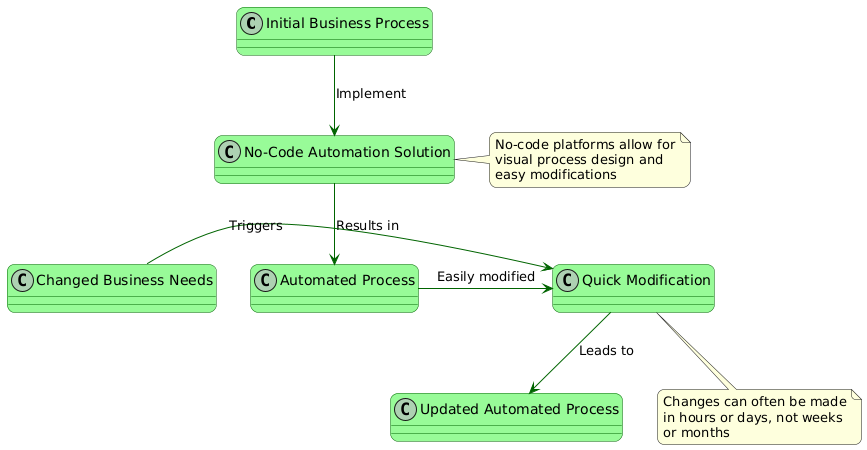
\includegraphics[width=0.75\textwidth]{figures/06-adaptability-no-code-solution}
    \caption{A flowchart showing the adaptability of a no-code automation solution, demonstrating how it can be easily modified as business needs change}
    \label{fig:06-adaptability-no-code-solution}
\end{figure}

\section{Implementation: Bringing Automation to Life}

Once the proposal is accepted, it's time to put your plan into action. Here's how to ensure a smooth implementation process:

\subsection{Setting Clear Expectations}

Start the implementation phase on the right foot:

\begin{itemize}
    \item Use a CRM like HubSpot or Salesforce to track all client communications and project details
    \item Implement a project management tool like Nifty.pm (which we highly recommend at Protomated) to keep all stakeholders aligned and informed
    \item Utilize tools like Asana or Trello for task management and progress tracking
    \item Set up regular video conferences using Zoom or Microsoft Teams for check-ins and demos
\end{itemize}

\subsection{Managing the Transition}

Guide the client through the change process:

\begin{itemize}
    \item Use change management tools like Whatfix or WalkMe to provide in-app guidance for new automations
    \item Implement feedback collection tools like SurveyMonkey or Google Forms to gather user input
    \item Utilize analytics tools like Google Analytics or Mixpanel to track usage and adoption of new automated systems
\end{itemize}

\subsection{Demonstrating Progress}

Keep the client engaged and confident throughout the implementation:

\begin{itemize}
    \item Use data visualization tools like Tableau or Power BI to create compelling progress reports
    \item Implement time-tracking tools like Toggl or RescueTime to quantify time savings from automation
    \item Utilize screen recording tools like Loom or Screencast-O-Matic for creating quick demo videos of completed automations
\end{itemize}

% TODO @screenshot: A sample project dashboard showing implementation progress, completed milestones, and realized benefits

\section{Training: Empowering Clients with Automation Know-How}

Effective training is crucial for the long-term success of any automation project. Here's how to ensure your clients can make the most of their new automated systems:

\subsection{Developing a Comprehensive Training Program}

Create a training plan that addresses various learning styles and needs:

\begin{itemize}
    \item Offer a mix of in-person workshops, video tutorials, and written documentation
    \item Develop role-specific training modules for different user groups
    \item Include both technical training on using the systems and strategic training on leveraging automation for business goals
\end{itemize}

\subsection{Hands-On Learning}

Encourage active participation in the learning process:

\begin{itemize}
    \item Conduct interactive workshops where users can practice with the new systems
    \item Set up a sandbox environment for risk-free experimentation
    \item Assign "homework" tasks to reinforce learning between sessions
\end{itemize}

\subsection{Creating Lasting Resources}

Develop resources that clients can refer back to after formal training ends, while being mindful of scope:

\begin{itemize}
    \item Create a concise yet comprehensive user manual using tools like Gitbook or Notion
    \item Develop a targeted FAQ document based on common questions during training, using a tool like Tettra or Confluence
    \item Set up a lightweight knowledge base using tools like Helpjuice or Document360, focusing on key processes and troubleshooting
    \item Clearly define the scope of documentation in your initial proposal to manage expectations and avoid scope creep
    \item Consider offering tiered documentation options, allowing clients to choose the level of detail they need
\end{itemize}

% TODO @screenshot: A sample page from a user manual, showing clear, step-by-step instructions for using an automated process

\section{Ongoing Support: Nurturing Long-Term Success}

The journey doesn't end with implementation and training. Here's how to provide ongoing support and continue delivering value:

\subsection{Proactive Maintenance and Optimization}

Stay ahead of potential issues and continuously improve the automation:

\begin{itemize}
    \item Schedule regular check-ins to review system performance
    \item Proactively suggest optimizations based on usage data and new capabilities
    \item Keep the client informed about new features or integrations that could benefit them
\end{itemize}

\subsection{Scaling and Adaptation}

Help clients evolve their automation strategy as their business grows:

\begin{itemize}
    \item Regularly reassess the client's business needs and goals
    \item Propose new automations or expansions of existing ones to meet changing needs
    \item Assist in integrating new tools or systems into the existing automation framework
\end{itemize}

\subsection{Continuous Learning and Improvement}

Foster a culture of ongoing learning and adaptation:

\begin{itemize}
    \item Offer periodic "refresher" training sessions
    \item Share case studies or success stories from other clients to inspire new ideas
    \item Encourage clients to join user communities or attend industry events to stay current
\end{itemize}

\section{Conclusion: Building Lasting Partnerships Through Automation}

As we've seen throughout this chapter, successfully implementing automation for clients is about much more than just technical know-how. It's about building trust, demonstrating value, and fostering a long-term partnership focused on continuous improvement and adaptation.

Remember, in today's rapidly changing technological landscape, the specific tools of automation will continue to evolve. Your true value as an IT consultant lies in helping clients navigate this changing landscape, keeping them agile and aligned with their business goals.

This is why at Protomated, we've specialized in core no-code tools that allow for rapid development and easy adaptation. As outlined in this book, we're here to support you as a "silent implementation partner," helping you deliver exceptional value to your clients.

By following the strategies outlined in this chapter, you'll be well-equipped to guide your clients through every stage of their automation journey, from initial skepticism to long-term success.

% TODO @qr: A QR code linking to additional resources on the Protomated website for IT consultants looking to partner or get additional support

\section{Action Items}

To put these ideas into practice:

\begin{itemize}
    \item Develop a "automation readiness" questionnaire to use during the prospecting phase
    \item Create a template for an automation proposal that addresses common objections
    \item Design a basic training program for a common automation scenario
    \item Set up a system for regular check-ins and optimization reviews with existing clients
\end{itemize}

Remember, every client's journey with automation will be unique. Stay flexible, keep learning, and always focus on delivering real, measurable value. Your success as an IT consultant in the age of automation depends on your ability to be a trusted guide, helping your clients navigate the exciting possibilities of this ever-evolving landscape.